% TODO May need rework.
Standards and technologies for web applications are being rapidly developed, and the boundaries for what is possible to achieve in a web application are being continously pushed by browser vendors and standards groups. Web based applications are today a viable alternative, unless the application is intended for mobile platforms or is in need of heavy graphics performance, such as for photo/video editing and games, or basically everywhere where sophisticated memory management is required. In \emph{Why Mobile Web Apps Are Slow} \cite{MobileApps:Online} it is argued how Javascript is not yet suitable for heavy performing applications but this is not an issue for this project, as it is not included in the product's nature or scope in any way.

Of relevance to Rymd, the Web Real-Time Communications (WebRTC) protocol \cite{WebRTC:Online} has become usable for arbitrary data streams in major browsers in 2014. Also of relevance, the still unfinalized Web Crypto API \cite{WebCrypto:Online} has become available in an experimental stage in recent months. The goals of Rymd has thus become technically viable in a web environment as of very recently.

The development of client side data storage in HTML5 is also an area that has become more stable and supported across browsers and vendors. Web applications can utilize offline storage like databases (WebSQL and IndexedDB), key value stores (Web Storage), and even offline caching with Application Cache \cite{OfflineWebApps:Online} in order to build completely offline applications with no requirements for internet access.

\section{Client-side storage}

Client-side storage is how arbitrary data can be persisted on disk by a web browser, accessible over an API. This is a general term for several separate but related APIs:

\begin{description}
  \item[Web Storage]\cite{WebStorage:Online} is a simple key-value store in the HTML5 specification.
  \item[WebSQL Database]\cite{WebSQL:Online} is an embedded SQL relational database.
  \item[FileSystem]\cite{FileSystem:Online} is an API providing direct file system access.
  \item[Indexed Database]\cite{IndexedDB:Online} is a NoSQL asynchronous data store.
\end{description}

All of these technologies offers ways of storing data on the user's hard drive instead of on a remote server. There are two main reasons for this: to make the application available offline, and to improve performance (fewer requests to a server). Older storage techniques include cookies, plugin based storage (Java, Flash, Google Gears), or browser-specific features.

All four APIs tie data to a single \emph{origin}, which is called \emph{Same Origin Policy}. An origin is the transfer protocol, the domain, and the port number. Thus every data store is associated with an origin, which implicates certain security aspects: an application in \emph{http://domain.com/subdir} may retrieve data from \emph{http://domain.com/subdir/dir} since they have the same origin, but cannot retrieve data from \emph{https://domain.com:3000} due to the different protocol and port number. This is a layer of protection against Cross Site Scripting (XSS) attacks, even though there is no prevention against XSS holes in the other parts of the application (the database might be compromised due to malicious scripts injected elsewhere).

In order to prevent malicious flooding of users' hard drives, browsers impose limits on storage capacity. If the application exceeds that limit the browser typically show a dialog in the interface to let the user increase the the limit. This quota is separated for each origin and storage mechanism. For instance, "sub.domain.com" may be allowed to store 5MB of Web Storage and 25MB of IndexedDB data, while "sub2.domain.com" may have other restrictions.

Both the database mechanisms, IndexedDB and WebSQL, supports \emph{transactions}. This ensures the integrity of the database due to the prevention of \emph{race conditions}, a phenomenon where two sequences of operations are applied at the same time, leading to unpredictable results and a database state of dubious accuracy.

Most of the storage formats supports synchronous and asynchronous modes. Synchronous mode is blocking, meaning that the storage operation will be executed and completed before the next line of code is executed. Asynchronous operations are non-blocking and performed in the background while the rest of the code is executed, and may be completed at a later stage. Generally a \emph{callback function} is provided, and is triggered on completion. This fits well with the asynchronous nature of Javascript, where events and callbacks are used heavily. The Javascript code snippets in listings~\ref{lst:syncCall} and \ref{lst:asyncCall} show the difference in synchronous and asynchronous calls.

\begin{Code}
\begin{lstlisting}[caption={Synchronous call}, label={lst:syncCall}]
// Fetch a record with id 10 from a database and store in variable
var result = DB.find(10);
\end{lstlisting}

\begin{lstlisting}[caption={Asynchronous call}, label={lst:asyncCall}]
/*
  Request a record with id 10 from a database, continue execute other code,
  and handle result of the database operation in callback when it has finished
*/
var request = DB.find(10);

request.onsuccess = function(evt) {
  var result = evt.result;
};
\end{lstlisting}
\end{Code}

% Mention WebSQL, IndexedDB, etc.
% TODO Johan

\subsection{Web Storage}

Web Storage is for persisting data in key-value pairs through a single object in web browsers. The API is as simple as attaching values as strings on properties of the global \texttt{localStorage} object as seen in figure~\ref{lst:localStorage}. The \texttt{localStorage} is persists data through browser sessions, while the \texttt{sessionStorage} object will clear all data when the browser tab or window is closed.

\begin{Code}
\begin{lstlisting}[caption={Use of Web Storage}, label={lst:localStorage}]
// Save an item in the local store
localStorage.foo = "bar";
// or
localStorage.setItem("foo", "bar");

// Retrieve item
var val = localStorage.foo;
// or
var val = localStorage.getItem("foo");

// Delete item
localStorage.removeItem("foo");
\end{lstlisting}
\end{Code}

\subsection{WebSQL}
\label{sec:websql}
WebSQL is the only client-side storage technology mentioned who tries to mimic a traditional SQL relational database. It comes with tables, indexing, transactions, keys and support for schemas. Regular SQL expressions are used to interact with the database, which means the developer can rely on the vast research that has been made in SQL query optimization. WebSQL is very performant thanks to indexing, and many database developers can start using it as-is. However, by the use of SQL the database is vulnarable to SQL injection attacks, unless this is taken into account by the developer.

\begin{Code}
\begin{lstlisting}[caption={Use of WebSQL}, label={lst:websql}]
// Create or open database with name, version, description and size of 2MB
var db = openDatabase('testdb', '1.0', 'Test database', 2 * 1024 * 1024);

// Create table and insert data
db.transaction(function(tx) {
  tx.executeSql('CREATE TABLE IF NOT EXISTS NAMES (id unique, first, second)');
  tx.executeSql('INSERT INTO LOGS (id, first, second) VALUES (1, "Johan", "Brook")');
});

// Retrieve all names and print them
db.transaction(function(tx) {
   tx.executeSql('SELECT * FROM NAMES', [], function(tx, results) {
     var len = results.rows.length, item;

     for (var i = 0; i < len; i++){
       item = results.rows.item(i);
       console.log("Name: " + item.first + " " + item.second);
     }
  }, null);
});
\end{lstlisting}
\end{Code}

\subsection{FileSystem}
\label{sec:filesystem}
The FileSystem API allows for creation and reading of files and folders on the user's hard drive. Currently, only Google Chrome has a working implementation of the API. FileSystem is suitable for storing larger binary files, and has good performance thanks to its asynchronous structure. There is no support for transactions or indexing. Its API includes methods for manipulating files and folders, as one would expect from a standard file system.

\begin{Code}
\begin{lstlisting}[caption={Use of FileSystem}, label={lst:filesystem}]
// Requesting a sandboxed, persistent file system with a size of 2MB and success callback
window.requestFileSystem(window.PERSISTENT, 2 * 1024 * 1024, function(fs) {
  console.log("Opened filesystem: " + fs.name);

  // Create a text file
  fs.root.getFile("test.txt", { create: true, exclusive: true }, function(fileEntry) {
    console.log("Created " + fileEntry.name + " in " + fileEntry.fullPath);
    // => "Created test.txt in /test.txt"
  });

  // Reading a file
  fs.root.getFile("test.txt", {}, function(fileEntry) {

    // Get a File object and read its contents with FileReader.
    fileEntry.file(function(file) {
      var reader = new FileReader();

      reader.onloadend = function() {
        var contents = this.result;

        console.log(contents);
      };

      reader.readAsText(file);
    });
  });

  // Other methods of FileEntry:
  fileEntry.getMetadata(successCallback, opt_errorCallback);
  fileEntry.remove(successCallback, opt_errorCallback);
  fileEntry.moveTo(dirEntry, opt_newName, opt_successCallback, opt_errorCallback);
  fileEntry.copyTo(dirEntry, opt_newName, opt_successCallback, opt_errorCallback);
  fileEntry.getParent(successCallback, opt_errorCallback);
  fileEntry.toURL(opt_mimeType);

  fileEntry.createWriter(successCallback, opt_errorCallback);
});
\end{lstlisting}
\end{Code}

\subsection{IndexedDB}
\label{sec:indexeddb}
The IndexedDB is a transactional, indexed client side database capable of storing different types of data structures with an asynchronous API. IndexedDB is actively developed and implemented in the latest versions of Mozilla Firefox, Google Chrome, Microsoft Internet Explorer and Opera: its specification is a Candidate Recommendation by the W3C, as of July 2013\cite{IndexedDB:Online}.

\subsubsection{Basic structure}
% Cursors, Object Stores, Indexes
Due to IndexedDB's object-oriented nature, a database includes a set of \emph{object stores}, which act similarly to tables in relational database management systems. An object store can hold \emph{objects} of different types, including binary data and Javascript primitives and objects. Each object has a \emph{key} (either specified by the developer from the object's properties, or automatically generated and managed by the database) that is used for indexing and retrieving records. One or several \emph{indexes} can be created on a store from an object's properties for quick querying. A \emph{cursor} is used to iterate on the resulting set of objects from a query on the store.

% Async API
% -----------
% Requests, Callbacks, Events, NoSQL
The asynchronous API might include complex patterns if the developer is not used to NoSQL structures. Unlike WebSQL, IndexedDB does not support SQL, and instead exposes ways for querying and manipulating data via \emph{requests} and \emph{transactions} (see section~\ref{subsec:security}). A positive facet of the rejection of SQL in favor of NoSQL is the prevention of SQL injection attacks, but at the cost of a steeper learning curve for already experienced database developers. Queries to the database will not yield the resulting data set: instead requests are returned, which will trigger \emph{events} for when the operation is finished. When an event is triggered a callback can be passed to handle the scenario and use the data.

\begin{Code}
\begin{lstlisting}[caption={Use of IndexedDB}]
var request = indexedDB.open("testdatabase");

// On database version migrations
request.onupgradeneeded = function(event) {
  var db = event.target.result;

  // Create an objectStore for this database
  var objectStore = db.createObjectStore("store");
};

// When the database is ready to use
request.onsuccess = function(event) {
  var db = request.result;

  // Insert "foo" in the store
  var insertTransaction = db.transaction(["store"], "readwrite").objectStore("store").put("Foo");

  insertTransaction.onsuccess = function(evt) {
    console.log("Inserted 'foo'");
  };

  // Read value with key "key" from the store
  var readTransaction = db.transaction(["store"], "read").objectStore("store").get("key");
  readTransaction.onsuccess = function(evt) {
    console.log("Found " + evt.target.result);
  };
};
\end{lstlisting}
\end{Code}

\subsubsection{Security and reliability}
\label{subsec:security}
IndexedDB is built on a transactional model, which means that all commands run inside a transaction context. Transactions have a certain lifetime, and cannot be used after its expiration. This transactional model is especially useful for when several instances of a client application are using the same database and issuing commands: without transactions, concurrency problems and other collisions might occur with data loss as a result. Transactions are able to abort and be rolled back to the state of the database before the transaction was started.

Kimak, Ellman and Laing highlight four important aspects of securing a IndexedDB driven application in their \emph{An Investigation into Possible Attacks on HTML5 IndexedDB and their Prevention}\cite{IndexedDBSecurity:2012:Online}:

\begin{itemize}
  \item Client side data encryption
  \item Input validation
  \item SOP (Same-Origin Policy)
  \item Code analysis
\end{itemize}

The database in IndexedDB does not include any kind of bundled encryption or validation, which means it is the developer's responsibility to sanitize and encrypt sensitive data before inserting into the store. Encryption is vital for the scenario where the contents of the database are compromised: the attacker must have access to the encryption key in order to read the information in plain text. Validation is needed if malicious content, such as Javascript, is inserted as the data fields in the store and then will be executed at a later stage.

Code analysis is divided into \emph{static} and \emph{dynamic} analysis. Static analysis is the analysis of the to-be insterted data in order to detect malicious material. Dynamic analysis is the analysis of executed programs, and can according to \cite{IndexedDBSecurity:2012:Online} be done by checking the call from the web application to the database and on success, the database operation can be performed.

\section{Distributed storage}
With the inherent problems of trust in CAs in a PKI, several approaches to publicly available distribution of cryptographic keys have emerged in recent years. Some use a blockchain-based approach derived from Bitcoin. This implies distributing a cryptographically based ledger over an entire network and taking it beyond that of a monetary currency to systems that can be used for a wider range of applications. There are also other ideas on how to solve the trust issue.

\subsection{Namecoin}
A phenomenon that has been on the rise during recent years is that of cryptocurrencies such as Bitcoin \cite{CryptoCoinInsider:2014:Online}. Each participant in the Bitcoin network keeps a ledger of all transactions throughout the history of the network. In order for a transaction to be deemed valid, it needs to be included in a cryptographically signed block together with a salt by one of the nodes, with a hash that has a special format. It is this brute-force search for salts that generates these hashes that are called \emph{mining} and constitute the work done by \emph{miners} to keep the network running. As an incentive, each verified block also includes a reward to the miner that first finds it and submits it to the blockchain\cite{internetForBeginners:2014:Online}. In effect, all transactions ever made are publicly available and tracked so that anyone can confirm their validity. This prevents forgery and double-spending of bitcoins.

Namecoin\cite{CryptoCoinInsider:2014:Online}, another cryptocurrency, is essentially a fork of Bitcoin with new transaction types that allows its blockchain to be utilized as a distributed key-value store. Although similar in nature to Bitcoin, its main purpose is to be used as a decentralized domain name system (DNS), rather than as a monetary currency.

With a decentralized DNS such as Namecoin, top level domains (such as \emph{.com} or \emph{.se}) can exist without being controlled by any central authority \cite{CryptoCoinInsider:2014:Online}. Also, the DNS lookup tables where domain names and their IP addresses are stored are shared in a peer-to-peer manner. The only necessary condition for these domains to be accessible is that there are participants willing to run the DNS server software. Although mainly intended to be used as a DNS, it contains several namespaces where arbitrary strings such as public cryptographic keys can be stored.

\subsection{Ethereum}
Bitcoin and its derivatives have a built-in scripting language that runs on top of the blockchain. It has limited functionality and is mainly used to set up contracts and multi-party-signed transactions that enables escrow-like functionality. Ethereum\cite{Ethereum:Online} is a novel crypto-currency built from scratch that extends this idea by building on \emph{smart contracts}, using a Turing complete domain specific language. This makes it a platform for buildig arbitrary distributed system. Users running code pay a small fee of the internal currency \emph{ether} for each computational step. Ethereum could therefore work not only as a DHT, but also execute parts of system logic. Development of Ethereum was started in 2013 and has a planned first release in late 2014.

\subsection{Keybase}
Keybase \cite{Keybase:Online} is another recent initiative that intends to solve the distribution of public keys. It is essentially a HTTP-interface that maps keys to identities. While keys themselves are stored centrally at Keybase's servers, it utilizes social media for proofs. The idea is that a Keybase user will put proofs of their Keybase identity on public social media services like Twitter or Github, and the Keybase client will refer to these to make sure that the given key corresponds to the user of these social media accounts. It ties identities to keys as long as a user's Keybase and social media accounts are not all compromised.

\section{Peer-to-Peer networking}

% Mention WebSockets, others?
% TODO Niklas & Robin

Up until recently browsers has lacked support for direct peer-to-peer communication. Then in 2011 Google released a project called WebRTC, with the purpose of enabling real-time voice and video in the browser \cite{WebRTCMemo:Online}.

Since the announcement of WebRTC, the organizations W3C and IETF have worked together on standarizing protocols, and drafing APIs. The major browser vendors Google, Mozilla and Opera support the project \cite{WebRTCAndMicrosoft:2012:Online}. While Microsoft actually supports the concept of WebRTC and contributes to the W3C WebRTC working group, it does not support Google’s (or nowdays, W3C’s and IETF) version of it\cite{WebRTCAndMicrosoft:2012:Online}.

Microsoft warns against supporting the new technology until it has actually become a standard and also does not fully agree on some constraints placed on the technology\cite{WebRTCAndMicrosoft:2012:Online}. Microsoft explains that one of their issues with the current WebRTC version is that it has predetermined paths for choosing codecs and ways of sending media over the network – sort of similar to a black box. This hinders application developers who want to optimize to suit their own needs. Microsoft’s answer to this is their own CU-RTC-WEB (Customizable, Ubiquitous Real Time Communication over the Web) which tries to addresses these issues.
% TODO, it seems like more than Google and Mozilla are involved in the project eg Opera
All in all, Microsoft remains optimistic that a common standard will eventually be established\cite{WebRTCAndMicrosoft:2012:Online}. They do however stress that more participants need to get involved in addition to Google and Mozilla. Since all major browser vendors (except Microsoft) support WebRTC at this time we chose this technology for the project.

\subsection{WebRTC}
WebRTC is a project which enables real-time communication between browsers\cite{WebRTC:Online}. Through the project, developers are able to create different types of applications which leverage peer-to-peer technology.

To obtain and transfer streaming data WebRTC's functionality is abstracted into three different APIs: \emph{MediaStream}, \emph{RTCPeerConnection} and \emph{RTCDataChannel}\cite{WebRTCBasics:2012:Online}. MediaStream, or \emph{getUserMedia}, handles synchronized media streams, i.e. synchronized video and sound from a computer's camera and microphone. RTCPeerConnection manages reliable and efficient communication of the data streams, it utilizes techniques such as \emph{jitter buffering} and \emph{echo cancellation} to ensure a high standard even in unstable networks. For the intent of file sharing, the RTCDataChannel API is the most relevant.

\subsubsection{RTCDataChannel}
The RTCDataChannel API allows for arbitrary data to be sent peer-to-peer by leveraging the RTCPeerConnection API. For the transportation of data, the API makes use of the SCTP (Stream Control Transport Protocol) protocol. SCTP is built on top on UDP, and provides some additional services such as congestion and flow control \cite{HighPerfBrowserNetworking:Online}.

Data transfers are secured with the DTLS (Datagram Transport Layer Security) protocol. The DTLS protocol is based on the TLS (Transport Layer Security) protocol, the main difference being that DTLS is constructed for datagrams while TLS is used for more reliable transport protocols such as TCP.

Before a connection can be initiated between peers, one of two parts must extend an offer which contains data describing the connection to the other part - this is often referred to as the signaling phase. The signaling phase requires a channel where the offer can be negotiated - it is usual for the channel to be a dedicated signaling server, but examples of a more serverless approach can be found\cite{webrtcsignalserver}. The standard does not provide any recommendations regarding the choice of signaling channel and protocol - this is for developers to decide. The connection phase is then handled by RTCPeerConnection which manages the ICE (Interactive Connectivity Establishment) workflow.

\subsubsection{NAT, STUN, TURN and ICE}
A problem with the construction of peer-to-peer applications using WebRTC, is the presence of NATs (Network Address Translation). NATs were first introduced in RFC 1631 as a short term solution to the problems regarding IP address depletion in IPv4. The idea was that by utilizing NATs, several hosts in a private network could together share a single public IP address \cite{RFC1631:Online}.

A NAT is responsible for maintaining a table with entries that map an internal IP address and port, to a public IP address and port and dropping these entries when they are no longer of relevance. When a host behind a NAT wants to communicate with an external host, the NAT creates an entry in the table, which can then be used to route the response back to the internal host(See figure ~\ref{fig:NAT}) \cite{RFC5245:Online}.

\begin{figure}[htp]
\centering
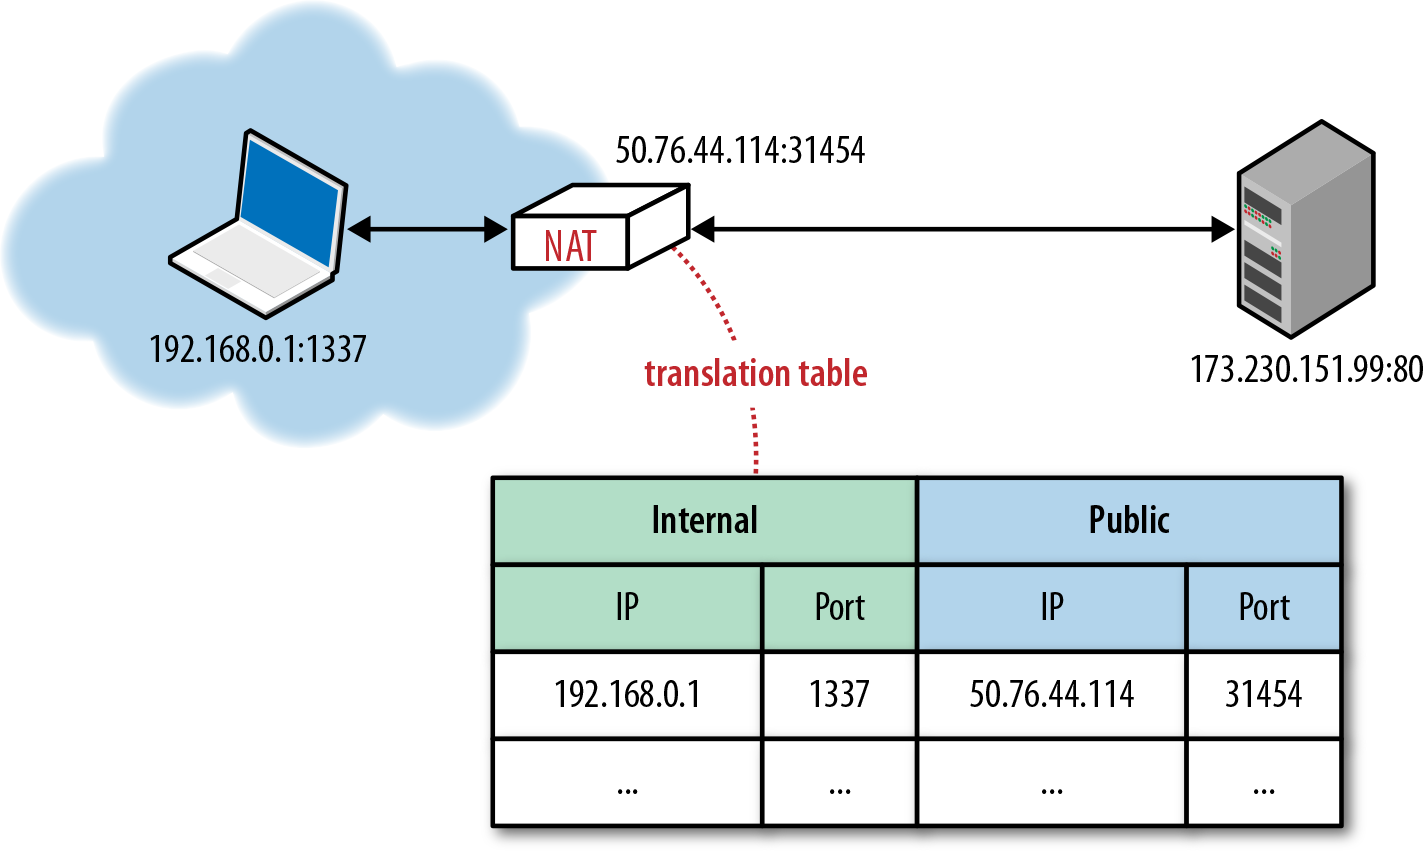
\includegraphics[width=\textwidth,height=0.2\paperheight,keepaspectratio
]{figures/nat}
\caption{A NAT maintains a table mapping internal IP and port, to a public IP and port. \cite{NATIllustration:Online}.}
\label{fig:NAT}
\end{figure}

The reason why the presence of NATs can pose a problem for peer-to-peer communication in the browser is that WebRTC mainly leverage the UDP protocol for transportation of data. The underlying issue with the UDP protocol is the absense of state, as opposed to the TCP protocol. The statelessness of the UDP protocol makes is difficult for a NAT to determine when a table entry is no longer relevant and should be dropped, which leads to the fact that UDP routing entries are expired based on time. If an entry is predeterminedly expired, it will cause inbound packets to be dropped, as they can not reach the source. In the case of TCP, which got a well defined state, it is inherently simple to determine when an entry should be dropped.

A technique commonly used to solve the problem regarding UDP entries expiring and being dropped, is to utilize keepalives at regular intervals, which is commonly referred to as \emph{UDP hole punching} \cite{UDPHolePunching:Online}.

An additional problem is that internal hosts know their internal IP, but not the public one. If a host runs an application, which communicates the IP as a part of the payload to hosts oustide of the private network, there would obviously be a missmatch if the internal IP is chosen. Therefore it is common to utilize a protocol called STUN (Session Traversal Utilities for NAT), which was introduced in RFC 5389. The protocol enables hosts to obtain its public IP address, with the help of an external STUN server (See figure~\ref{fig:WebRTC - STUN}) \cite{RFC5389:Online}.

\begin{figure}[htp]
\centering
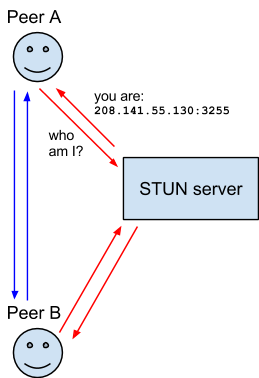
\includegraphics[width=\textwidth,height=0.2\paperheight,keepaspectratio
]{figures/webrtc-stun}
\caption{STUN servers let peers in a private network behind firewalls discover their public IP-addresses\cite{WebRTCArchitecture:2014:Online}.}
\label{fig:WebRTC - STUN}
\end{figure}

These techniques are not always adequate, which is caused by the fact that STUN does not work with all types of NATs, and in some cases UDP traffic might be blocked by a firewall. In these cases the TURN (Traversal Using Relays around NAT) protocol, specified in RFC 5766, can be leveraged.  TURN establish a TCP connection with a relay server in those cases where UDP fails. The relay server is used to tunnel data to the other host, which means that there is no longer a direct peer-to-peer connection (See figure~\ref{fig:WebRTC - TURN}) \cite{RFC5766:Online}.

\begin{figure}[htp]
\centering
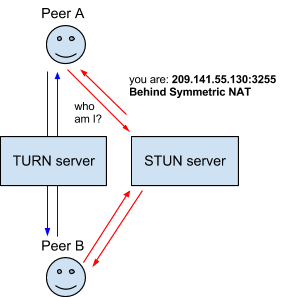
\includegraphics[width=\textwidth,height=0.2\paperheight,keepaspectratio
]{figures/webrtc-turn}
\caption{If a peer-to-peer connection cannot be established, a relay through a TURN server could be used. All peers send their packets through the relay which makes it more costly. But at least the connection works\cite{WebRTCArchitecture:2014:Online}.}
\label{fig:WebRTC - TURN}
\end{figure}

In the case of WebRTC, the techniques desribed above are leveraged through the ICE (Interactive Connection Establishment) protocol which is used by the RTCPeerConnection API. The ICE protocol is specified by RFC 5245 and has the objective of connecting peers in the most efficient way and it makes use of STUN and fallback to TURN when no other alternatives exists (See figure ~\ref{fig:ICE}) \cite{RFC5245:Online}.

\begin{figure}[htp]
\centering
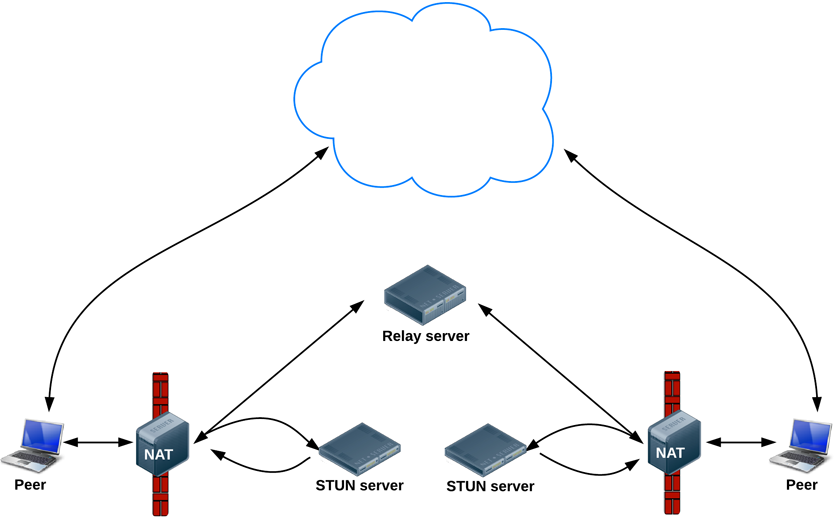
\includegraphics[width=\textwidth,height=0.25\paperheight,keepaspectratio
]{figures/ICE}
\caption{The different ways for ICE to find network interfaces and ports \cite{WebRTCBasics:2012:Online}}
\label{fig:ICE}
\end{figure}

\section{Cryptography}
Until recently, the practice of performing cryptographic operations in a web browser environment has been considered bad practice by security professionals\cite{Matasano:Online}. One reason for this is that it has been impossible to verify the integrity of client side source code between executions - something that has now changed with the advent of signed browser extensions. Another issue is the internal openness of JavaScript - any cryptographic implementation would unavoidably expose all their primitives, as well as raw private and secret key data. This is being addressed by the new Web Cryptography API\cite{WebCrypto:Online}, an open standard for implementation of cryptographic primitives in web clients accessible through client code. Basically, all primitives (such as hashing, encryption, decryption, signing and generation of keys) and raw key material would be black boxed for the client application and executed natively in the web browser. However, it is not yet finished and at this time of writing only Google Chrome out of the major browsers have implemented more than a basic pseudo-random number generator.

\subsection{Web Crypto API}
The Web Crypto API provides a common set of interfaces that allow rich web applications to preform signature generation and verification, hashing and verification, encryption and decryption, without requiring access to the raw material. The Web Crypto Api is still in an early implementation stage and the exact implementation of the different functionalities may come to change many times over time.

\subsection{Certificates} % wikipedia
In essence, a certificate contains a public key plus additional information about the user and: Usually the whole block is signed by a Central Authority) or another third party, the signing helps to prof the identity.
One commonly used schema for certificates is the X.509 standard. In the X.509 system, a (CA) issues a certificate, binding a public key to a name such as an e-mail address or a DNS entry.

\subsection{Advanced Encryption Standard}
AES is based on the idea of substitution-permutation\cite{AESISFAST:Online}, this supports that
diffusion and confusions together will complicate statistics attacks and hides local patterns in the language. Unlike DES who uses a Fiestel network, AES is using a structure  similar to Rijndael – with a fixed block size. Encryption is done with the same key but inversed. The algorithm described by AES is a symmetric-key algorithm, meaning the same key is used for both encrypting and decrypting the data.
